\chapter{Конструкторский раздел}
В данном разделе описываются основные шаги выполнения SQL-запроса в СУБД. Приводится алгоритм построения запроса планировщиком PostgreSQL, его стоимостная модель. Представлено описание запроса в исчислении предикатов и его сравнение с SQL версией. Излагаются подходы к распараллеливанию SQL-запросов, плана запроса и выделение независимых частей последовательности предикатов.

\section{Основные шаги выполнения SQL-запроса}
\vspace{-0.5cm}
Основные шаги, которые выполняются при выполнении SQL-запроса в реляционных СУБД, представлены на рисунке \ref{image:query_plan} \cite{stages_sql_query}.

\begin{figure}[H]
	\captionsetup{justification=centering}
	\centering{
		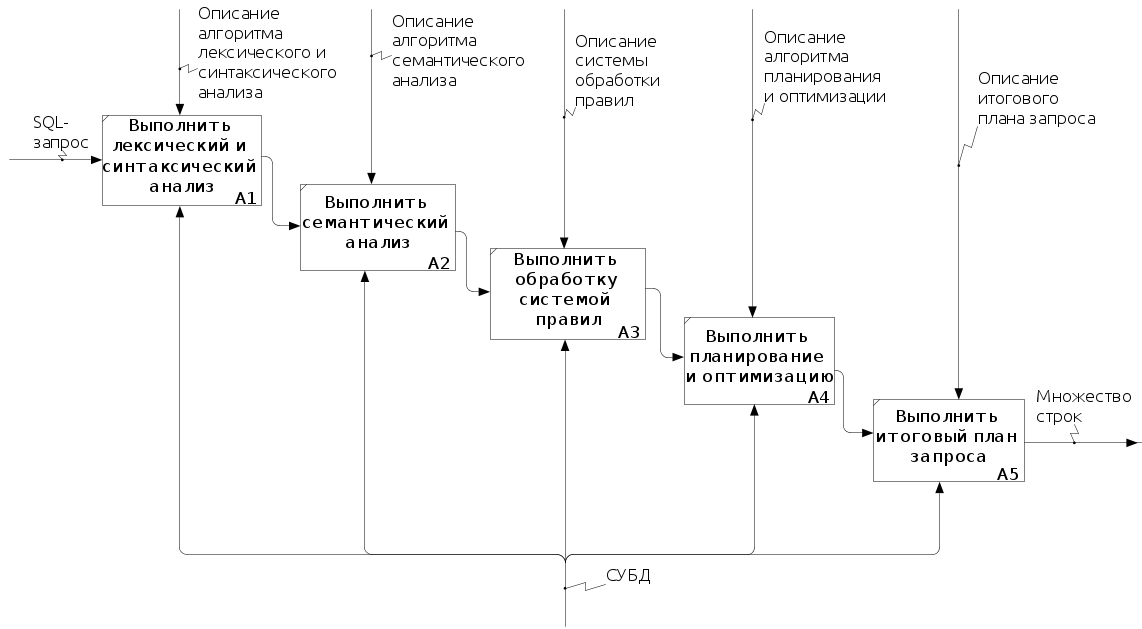
\includegraphics[scale=0.41]{./images/stages_plan_sql.png}
		\caption{Выполнение запроса в СУБД.}
	    \label{image:query_plan}
    }
\end{figure}

\begin{enumerate}
	\item Лексический и синтаксический анализ. Входная строка пользователя обрабатывается лексическим и синтаксическим анализаторами; в результате строится дерево запроса.
	\vspace{-0.2cm}
	\item Семантический анализ. Полученное дерево запроса дополняется различного рода метаинформацией: системными идентификаторами таблиц, типами и порядковыми номерами запрашиваемых полей, перечнем соединяемых таблиц и т.д.
	\vspace{-0.2cm}
	\item Обработка системой правил. Выполняется поиск в системных каталогах правил, применимых к дереву запроса, и при обнаружении подходящих выполняются преобразования, которые описаны в теле найденного правила.
	\vspace{-0.2cm}
	\item Планирование и оптимизация. На вход планировщику поступает структура с деревом запроса (рисунок \ref{image:parse_query_tree}). Осуществляется выбор наиболее эффективного пути выполнения этого запроса с точки зрения имеющихся оценок затрат и статической информации на момент выполнения.  После выбора оптимального метода доступа к данным, конечный вариант преобразуется в полноценный план запроса и передается исполнителю. 
	\vspace{-0.2cm}
	\item Выполнение итогового плана запроса. Исполнителем осуществляется рекурсивный обход по дереву плана: \textit{сканируются отношения}, выполняется \textit{сортировка} и \textit{соединения}, вычисляются \textit{условия фильтра} и др. После выполненных этапов возвращается результирующее множество строк.
\end{enumerate}

\section{Алгоритм построения запроса в PostgreSQL}
\vspace{-0.5cm}
В аналитическом разделе была рассмотрена работа планировщика на верхнем уровне. Теперь же стоит заглянуть более детально в каждый из разделов и выяснить, как обрабатывается запрос, содержащий простые операторы SELECT, FROM, WHERE. 

Алгоритм построения запроса в PostgreSQL представлен следующим образом: на  рисунке \ref{image:dfd_level_1} -- более подробно описаны шаги выполнения, необходимы для модификации основной части; рисунок \ref{image:dfd_level_2} отражает этапы предварительной обработки создания основного плана запроса; рисунок \ref{image:dfd_level_3} представляет непосредственно базисные функции для выбора оптимального пути \cite{source_code_postgresql, help_understanding_code}.
\clearpage
\begin{figure}[ht!]
	\captionsetup{justification=centering}
	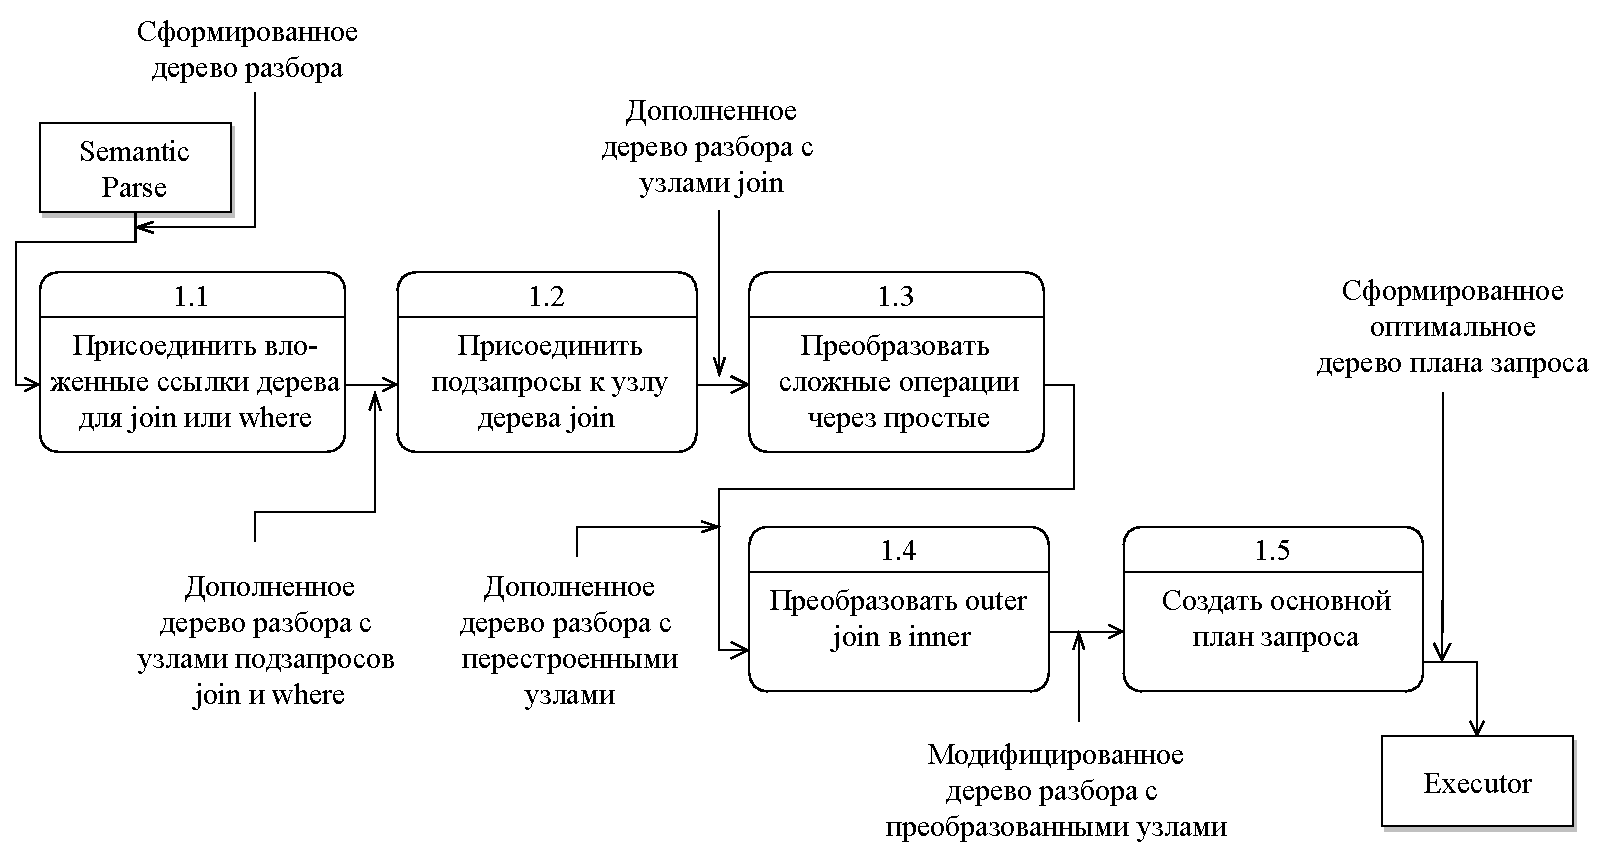
\includegraphics[scale=0.6]{images/dfd_level_1}
	\caption{Шаги выполнения планировщика и оптимизатора}
	\label{image:dfd_level_1}
\end{figure}	
\begin{figure}[ht!]
	\captionsetup{justification=centering}
	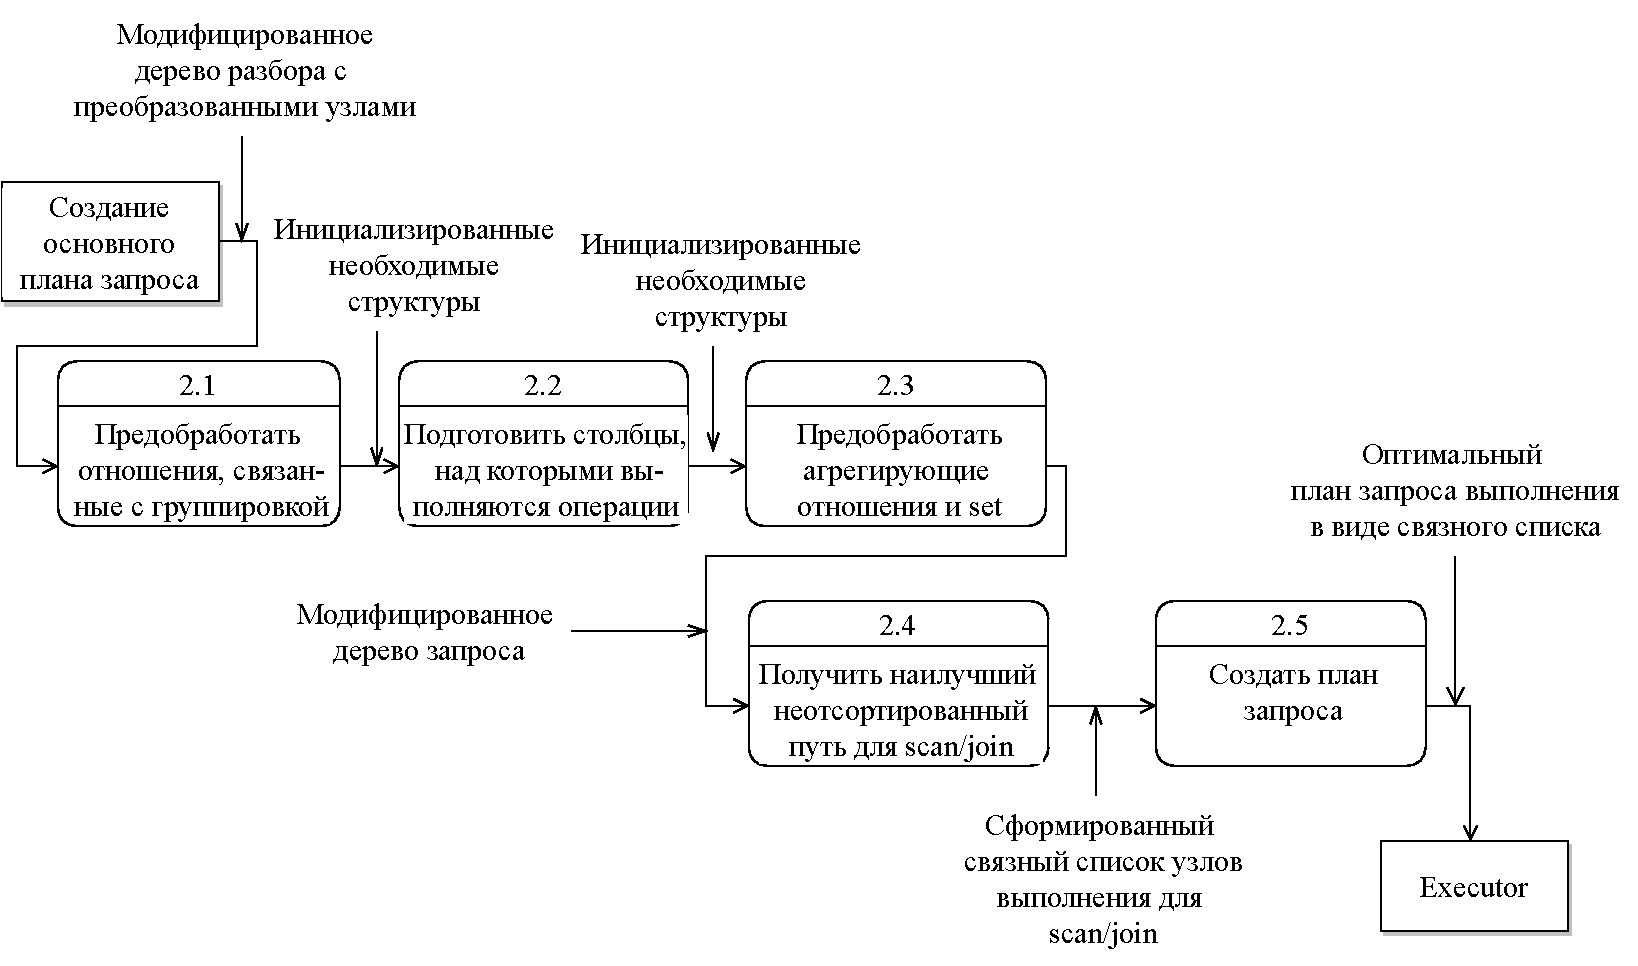
\includegraphics[scale=0.6]{images/dfd_level_2}
	\caption{Шаги выполнения предварительной обработки для создания основного плана запроса}
	\label{image:dfd_level_2}
\end{figure}
\clearpage
\begin{figure}[ht!]
	\captionsetup{justification=centering}
	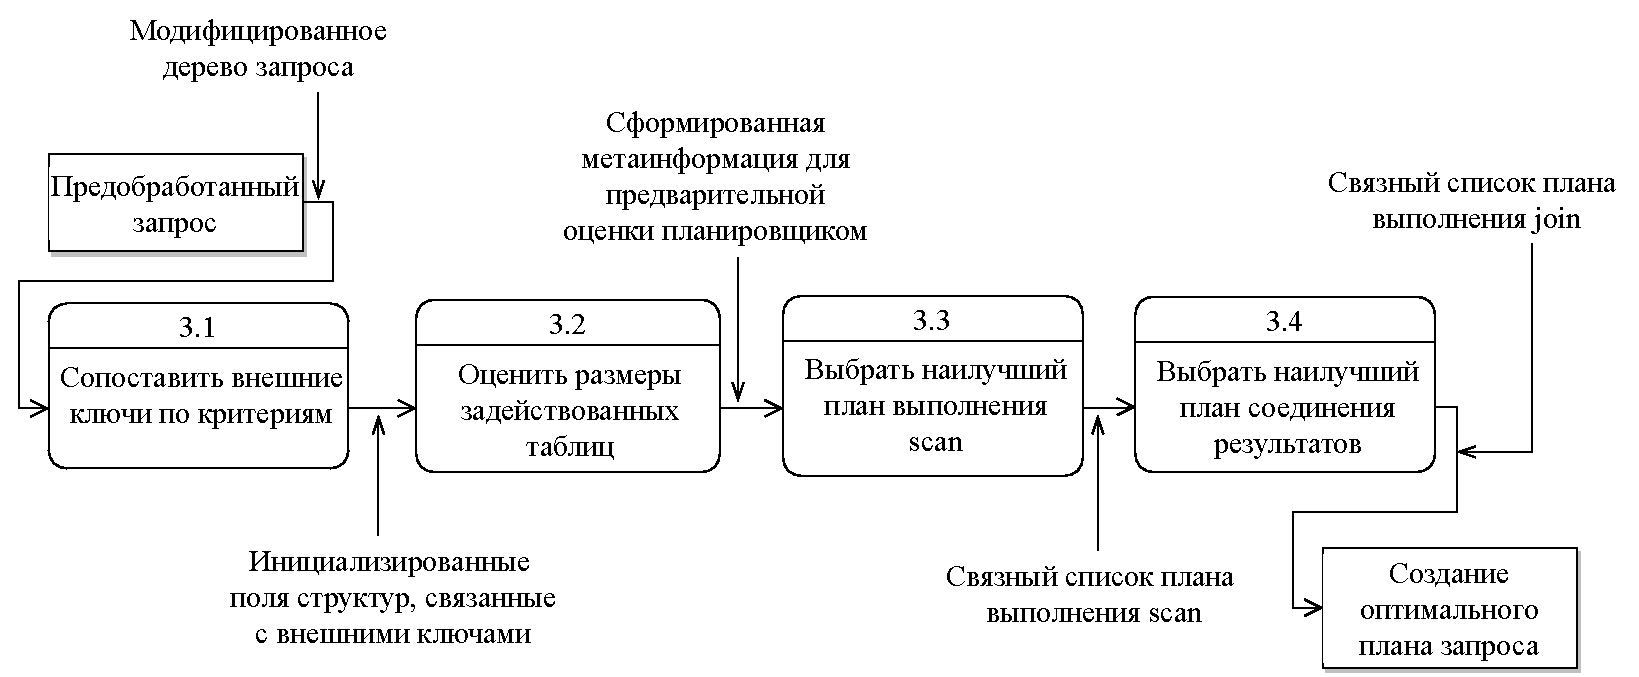
\includegraphics[scale=0.6]{images/dfd_level_3}
	\caption{Оценка и создание плана итогового запроса из оптимальных планов его узлов}
	\label{image:dfd_level_3}
\end{figure}

В процессе выбора наилучшего пути выполнения scan (3.3) выполняются действия по сравнению стоимости из учета выполнения и статистики следующих основных способов сканирования:
\begin{itemize}
	\item[$\circ$] \textit{sequential scan} -- последовательное сканирование всех строк таблицы. Если был найден результат в виде одной записи вначале, то операция поиска будет продолжена; \vspace{-0.2cm}
	\item[$\circ$] \textit{index scan} -- сканирование осуществляется путем использования индекса и, обычно, обхода B-дерева;\vspace{-0.2cm}
	\item[$\circ$] \textit{index only scan} -- аналогично выполнению index scan за исключением того, что данные извлекают из индекса, а не из самой таблицы;\vspace{-0.2cm}
	\item[$\circ$] \textit{bitmap scan} -- служит для поиска по нескольким индексам одновременно. Состоит из двух частей:\vspace{-0.2cm}
	\begin{itemize}
		\item \textit{bitmap index scan} -- читает индекс и строит битовую карту;\vspace{-0.2cm}
		\item \textit{bitmap heap scan} -- читает табличные страницы, используя построенную карту и др.\vspace{-0.2cm} 
	\end{itemize}
\end{itemize}

Процесс выбора наилучшего пути выполнения join (3.4) выполняет аналогичные действия, что и процесс 3.3, но связанные с объединением результатов:
\begin{itemize}
	\item[$\circ$] \textit{hash join} -- создается хэш-таблица на основе меньшей таблицы с ключом из join, загружая ее при этом в память целиком (если это возможно). Затем сканируется другие множества кортежей, и осуществляется проверка этой хэш-таблицы с внешней по ключам, используемым в соединении. Предпочтительно использовать в случае, когда обе таблицы содержат более 1000 записей, и используется оператор равенства.
	\vspace{-0.2cm}
	\item[$\circ$] \textit{merge join} -- выполняет объединение двух таблиц путем <<слияния>> -- объединения записей одной таблицы с записями из другой; при этом лучше, чтобы данные были отсортированными по ключу; используется, когда кортежи могут быть отсортированы наилучшим способом по сравнению с другими методами;  
	\vspace{-0.2cm}
	\item[$\circ$] \textit{nested loop join} -- для каждой строки первой таблицы выполняется сравнение с каждой строкой из второй на предмет совпадения ключей; используются, когда условие сравнения не содержит оператор равенства.
\end{itemize}

\section{Выполнение планировщиком PostgreSQL \newline JOIN-запроса}
\vspace{-0.5cm}
На примере PostgreSQL работа планировщика запросов для одной таблицы выглядит следующим образом \cite{plan_query_postgres}.
\begin{enumerate}
	\item Выполнение предварительной обработки. 
	\vspace{-0.2cm}
	\item Оценка всевозможных путей доступа к данным. Оцениваются затраты на последовательный доступ (\textit{seq scan}), сканирование индексов (\textit{index scan}), \textit{bitmap scan}; затем выполняется сортировка (\textit{sort}) или присоединение данных (\textit{join}).
	\vspace{-0.2cm}
	\item Выбор кратчайшего пути по затратам.
\end{enumerate}

При увеличении числа таблиц, участвующих в запросе, к основному алгоритму добавляются шаги. Процесс получения <<дешевого>> доступа к данным приведен на рисунке \ref{image:data_access}.
\begin{figure}[H]
	\captionsetup{justification=centering}
	\centering{
		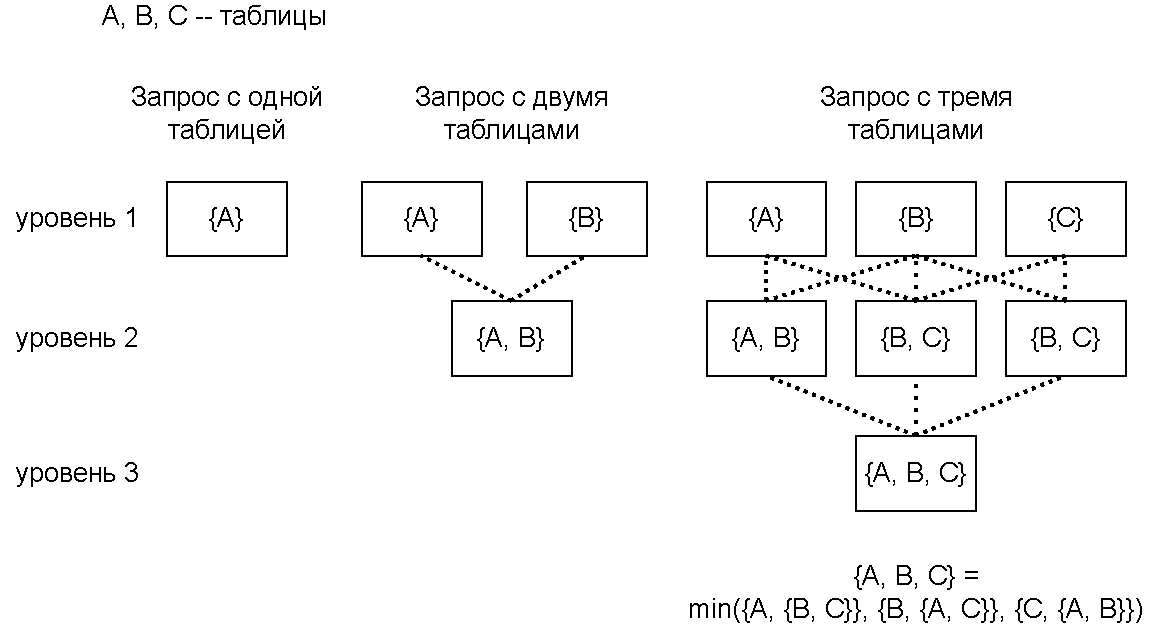
\includegraphics[scale=0.8]{./images/postgre_plan.pdf}
		\caption{Получение <<дешевого>> доступа к данным.}
		\label{image:data_access}
	}
\end{figure}

\begin{itemize}
	\item[$\circ$] Уровень 1. Найти кратчайший путь выполнения запроса для каждой таблицы.\vspace{-0.2cm}
	\item[$\circ$] Уровень 2. Получить самый кратчайший путь для каждой комбинации, в которой которой выбирается две таблицы из всех.\vspace{-0.2cm}
	\item[$\circ$] Уровень 3. Продолжить ту же обработку, пока в результате число таблиц не станет равным текущему уровню.\vspace{-0.2cm}
\end{itemize}

Для получения оптимального дерева плана запроса, планировщик должен рассмотреть комбинации всех индексов и возможности методов объединения. При увеличении числа используемых таблиц может наступить <<комбинаторный взрыв>>. Таким образом, при количестве таблиц, большем 12, используются \textit{генетические алгоритмы} \cite{generetic_algorithm}.

\section{Стоимостная модель PostgreSQL}
\vspace{-0.5cm}
В качестве критерия выбора единственного плана запроса из некоторого множества в движках СУБД таких, как PostgreSQL, MySQL и др., используется стоимостная модель. Само понятие <<стоимость>> отражает абстракцию сравнения выбора того или иного узла при построении результирующего дерева  \cite{postgres_explain}. Если запрос может быть построен несколькими способами, то будет выбран тот, который имеет наименьшую стоимость. В такой модели каждая вершина дерева плана может иметь один следующих параметров, приведенных в таблице \ref{table:cost_plan}. Все заданные коэффициенты являются относительными $seq\_page\_cost$.

\begin{table}[ht!]
	\centering
	\captionsetup{singlelinecheck = false, justification=raggedright}
	\caption{Сравнение основных характеристик СУБД}
	\label{table:cost_plan}
	\begin{tabular}{|c|c|c|c|}
		\hline 
		Обозначение & Коэффициент & Значение & Описание\\ \hline
		\multirow{3}{*}{$c_{s}$}	   & \multirow{3}{*}{seq\_page\_cost} & \multirow{3}{*}{1.0} & Чтение одной страницы \\ 
		& &  & с диска в серии \\
		& & & последовательных чтений \\ \hline
		\multirow{2}{*}{$c_{r}$} & \multirow{2}{*}{random\_page\_cost} & \multirow{2}{*}{4.0} & Чтение одной произвольной \\
		& & & страницы с диска \\ \hline
		\multirow{2}{*}{$c_{t}$}	   & \multirow{2}{*}{cpu\_tuple\_cost} & \multirow{2}{*}{0.01} & Обработка каждой строки \\ 
		& &  & при выполнении запроса \\ \hline
		\multirow{3}{*}{$c_{i}$}	   &  & \multirow{3}{*}{0.01} & Обработка каждой записи \\ 
		&  cpu\_index\_ &  & индекса при выполнении \\ 
		& tuple\_cost&  & запроса \\ \hline
		\multirow{2}{*}{$c_{o}$}	   & \multirow{2}{*}{cpu\_operator\_cost} & \multirow{2}{*}{0.0025} & Обработка оператора \\ 
		& &  & или функции \\ \hline
	\end{tabular}
\end{table}
Стоимость узла верхнего уровня включает стоимость всех его потомков. Она отражает только те факторы, которые учитывает планировщик, и не зависит от времени, которое необходимо для передачи результирующих кортежей клиенту. Общая стоимость вычисляется по формуле (\ref{eq:genercost}):

\vspace{-0.5cm}
\begin{equation}
	\label{eq:genercost}
	n_{s}c_{s} + n_{r}c_{r} + n_{t}c_{t} + n_{i}c_{i} + n_{o}c_{o}	
\end{equation}

\section{Описание запроса на логическом ЯП}
\vspace{-0.5cm}
Для представления утверждений (по аналогии с кортежами из реляционного подхода) в логике предикатов используются кванторы. Их можно рассматривать как краткие обозначения. Например, выражение $(\forall x)\ P(x)$ обозначает <<для каждого х высказывание P(x) истинно>>, а $(\exists x)\ P(x)$ -- <<существует такой х, что высказывание P(x) истинно>>. Это можно представить в виде формул (\ref{eq:forall}) и (\ref{eq:exists}):
\begin{equation}
	\label{eq:forall}
	(\forall x)\ (P(x)) \equiv (P(d_0) \land P(d_1) \land ... \land P(d_n))
\end{equation}
\begin{equation}
	(\exists x)\ (P(x)) \equiv (P(d_0) \lor P(d_1) \lor ... \lor P(d_n)),
	\label{eq:exists}
\end{equation}

где $\{d_0,...,d_n\}$ -- домены. Формулы (\ref{eq:forall}) и (\ref{eq:exists}) позволяют составлять запросы к хранилищам данных на основе математического аппарата, используя исчисление предикатов первого порядка.


\section{Логические запросы и запросы SQL}
\vspace{-0.5cm}
Декларативная парадигма программирования основывается на спецификации решения задачи, то есть описание проблемы и ожидаемого результата. Такой подход удобен, так как предоставление общих инструкций является более наглядным и простым методом по сравнению с формулированием цели в императивном стиле. 

Данная идея заложена в основе языка SQL. Для получения результата необходимо описать такую последовательность действий, которая позволит извлечь или модифицировать данные -- в данном случае это кортеж.

Для формального описания задачи логическое программирование использует логику предикатов \cite{logic_approach}. Такой стиль позволяет на основе заданных фактов и правил вывода получить новую информацию из исходной.

Существует некоторое отличие в представлении данных в виде отношения и предикатов логических языков: в первом случае нельзя хранить какие-то вложенные структуры. Напротив, аргументы предикатов могут быть сколь угодно сложными \cite{compare_relations_and_predicates_keeping}.

\section{Подходы к распараллеливанию SQL-запросов}
\vspace{-0.5cm}
Параллельная обработка запроса направлена на разделение одной большой задачи на небольшие, выполняющиеся в разных потоках. Благодаря такому способу сокращается время отклика системы для операций с интенсивным использованием данных, например, в хранилищах или в системах поддержки принятия решений (DSS).

Выделяют различные подходы, в которых можно выполнить распараллеливание SQL запроса \cite{parallel_query}:
\begin{itemize}
	\item[$\circ$] уровень доступа -- tables scan, index full scans,  partitioned index range scans;
	\vspace{-0.2cm}
	\item[$\circ$] уровень присоединения -- nested loop/merge/hash join; \vspace{-0.2cm}
	\item[$\circ$] DDL операции -- create, drop, alter; \vspace{-0.2cm}
	\item[$\circ$] DML операции -- select, insert, update. \vspace{-0.2cm}
\end{itemize}
Если модуль данных не является разделяемым, то выполняются следующие шаги:
\begin{enumerate}
	\item Разделение всех отношений, которые используются в запросе. \vspace{-0.2cm}
	\item Назначение отдельной группы отношений процессору (вместе с его модулем памяти). \vspace{-0.2cm}
	\item Перемещение промежуточного результирующего набора другому процессору для оценки результата. \vspace{-0.2cm}
\end{enumerate}
Стоит отметить, что данный метод применим только для операции select.

\vspace{-0.5cm}
\section{Подходы к распараллеливанию плана запроса}
\vspace{-0.5cm}
Немаловажную роль играют сами узлы построенного планировщиком дерева плана запроса. В основе идеи ускорения лежит обработка одновременно тех частей, которые до момента своего завершения не позволяют перейти на другой узел выполнения (в случае последовательной реализации) \cite{parallel_nodes_1}. Графически данный способ представлен на рисунке \ref{image:parallel nodes_1}.
\begin{figure}[H]
	\centering{
		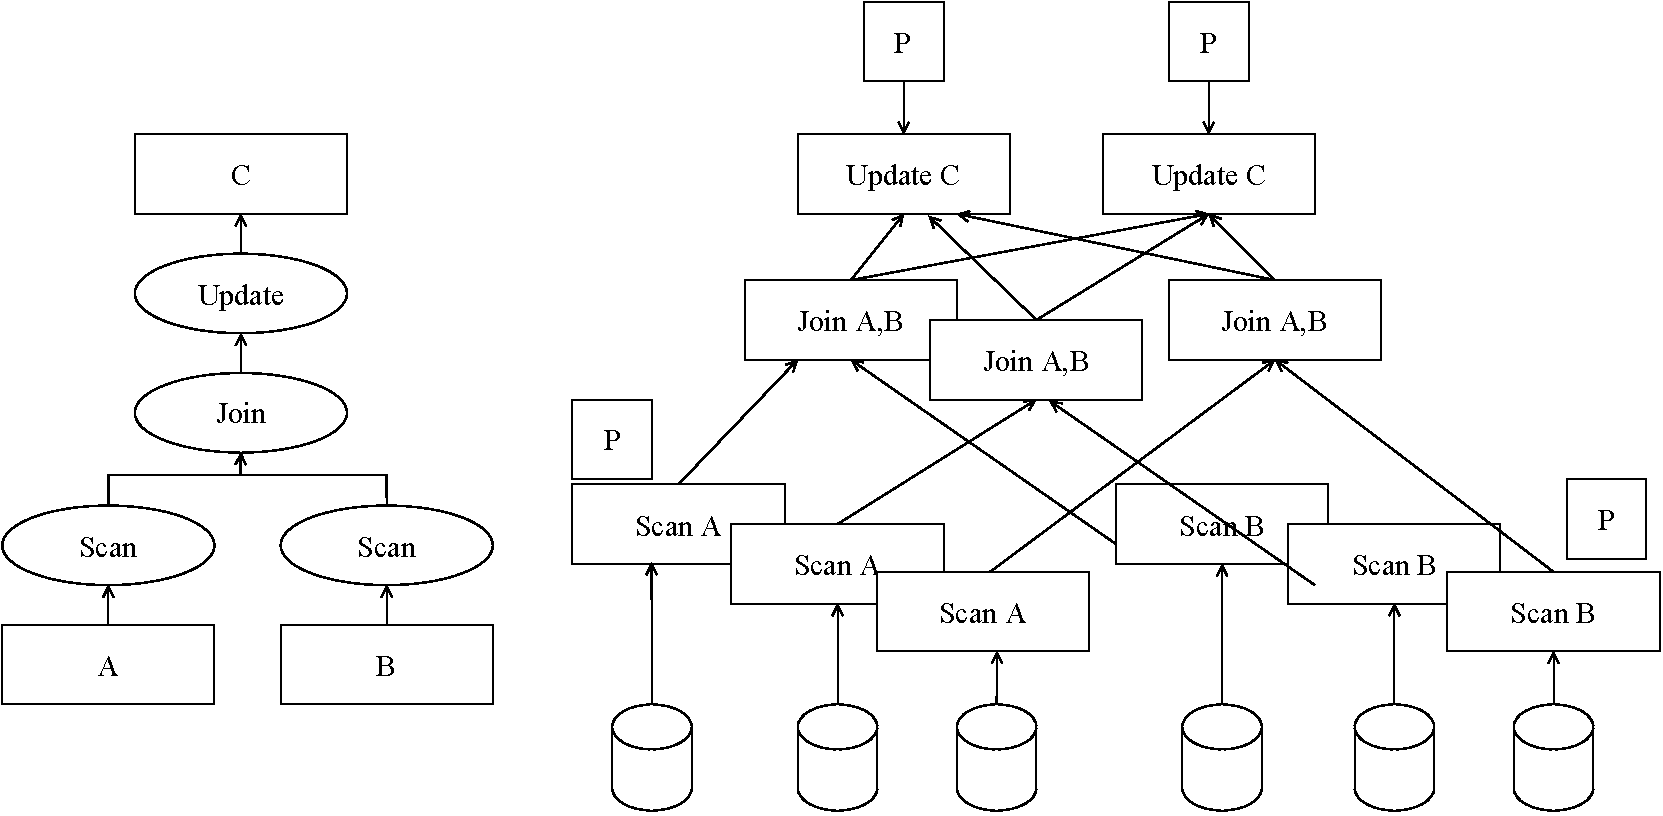
\includegraphics[scale=0.52]{./images/parallel_nodes.pdf}
		\caption{Узлы планировщика как идея для распараллеливания.}
		\label{image:parallel nodes_1}
	}
\end{figure}

\vspace{-0.5cm}
\section{Выделение независимых частей логического запроса}
\vspace{-0.5cm}
Рассмотрим запрос $(\forall v_i)(\forall p)(P \land B_1\land...\land B_n \rightarrow A)$, где 
\newline $P, B_1,...,B_n$ -- независимые предикаты, а $v_i, p$ -- переменные, относящиеся к ним. В случае логических языков программирования отдельное внимание уделяется обработке таких предикатов. Пусть для предиката $P$ время поиска ответа больше по сравнению с последующими из данной конъюнкции. Тогда системе приходится ждать, пока найдется такое решение (или его может не быть), чтобы перейти к дальнейшим шагам выполнения. Возникает вопрос о независимой и одновременной обработке таких предикатов.

Для решения данной проблемы выделяют следующие подходы \cite{and_or_parallelism}.
\begin{enumerate}
	\item AND-параллелизм (независимый).
	\vspace{-0.2cm}
	\item OR-параллелизм (независимый).
\end{enumerate}

Рассмотрим более подробно каждый из них.
\begin{itemize}
	\item[$\circ$] В основе идеи независимого AND-параллелизма лежит распараллеливание конъюнкции подцелей, которые не имеют одни и те же переменные. Такие термы не будут влиять на выполнение друг друга, устраняя необходимость введения какой-либо формы синхронизации во время параллельного выполнения. Данный способ проиллюстрирован на рисунке \ref{image:and_tree}.
	\begin{figure}[H]
		\centering{
			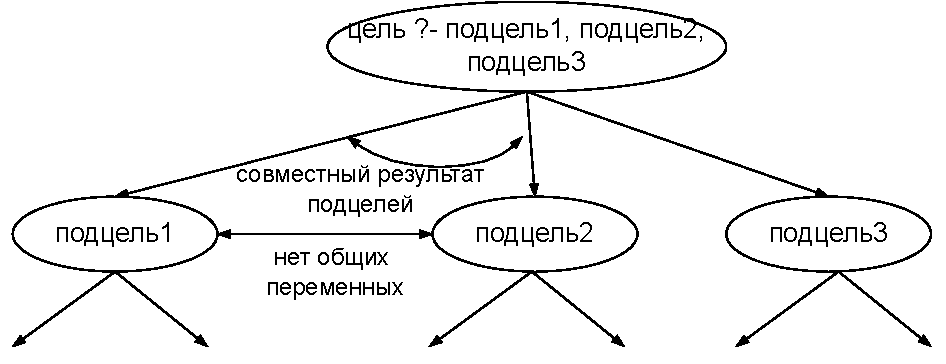
\includegraphics[scale=0.82]{./images/and_tree.pdf}
			\caption{AND-дерево.}
			\label{image:and_tree}
		}
	\end{figure}
	
	\item[$\circ$] Независимый OR-параллелизм основан на параллельном выполнении дизъюнкции предикатов, не имеющих общих переменных. Результат будет получен из первого выполнившегося терма. Пример OR-дерева приведен на рисунке \ref{image:or_tree}.
	\begin{figure}[H]
		\centering{
			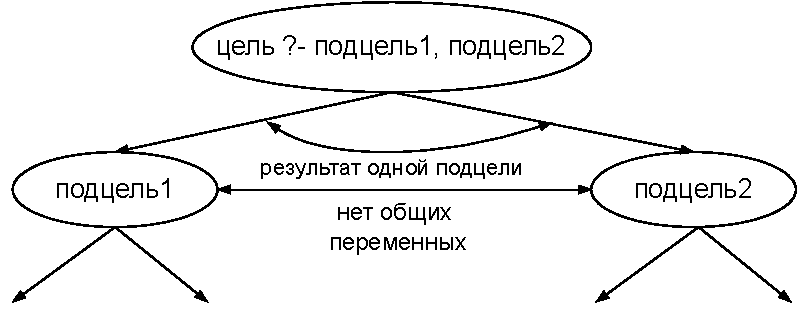
\includegraphics[scale=0.82]{./images/or_tree.pdf}
			\caption{OR-дерево.}
			\label{image:or_tree}
		}
	\end{figure}
\end{itemize}

\section*{Вывод}
\vspace{-0.5cm}
В данном разделе были описаны основные шаги выполнения SQL-запроса в СУБД. Приведен алгоритм построения запроса планировщиком PostgreSQL, его стоимостная модель. Представлено описание запроса в исчислении предикатов и его сравнение с SQL версией. Были изложены подходы к распараллеливанию SQL-запросов, плана запроса и выделение независимых частей последовательности предикатов.